\documentclass{article}

\usepackage{booktabs}
\usepackage{tabularx}
\usepackage{pdfpages}

\title{SE 3XA3: Development Plan\\MovieGuide}

\author{Team 35, PGH Software Solutions
		\\ Pratyush Bhandari and bhandarp
		\\ Gazenfar Syed name and syedg1
		\\ Hamid Ghasemi, ghasemih
}

\date{}

\input{../Comments}

\begin{document}

\begin{table}[hp]
\caption{Revision History} \label{TblRevisionHistory}
\begin{tabularx}{\textwidth}{llX}
\toprule
\textbf{Date} & \textbf{Developer(s)} & \textbf{Change}\\
\midrule
Sept 28th & Pratyush & Put together latex document\\
Sept 27th & Gazenfar, Hamid & Wrote different points for development plan\\
\bottomrule
\end{tabularx}
\end{table}

\newpage

\maketitle

The following document will concisely go through the different aspects of our development plan. Each different aspect will be broken up into its respective section.

\section{Team Meeting Plan}
Our team meeting plan involves meeting twice a week in lab. We aim to utilize this time as much as possible to discuss progress and formulate objectives. Furthermore, we will be setting up weekly meetings outside of class to work on the deliverables collaboratively. Each week we will take turns being the ?chair? of the meeting. The chair will be responsible to go over the sub-tasks for each deliverable and will document meeting notes.

\section{Team Communication Plan}
We will primarily be using facebook to communicate with each other. We have created a group chat where we will discuss anything related to the project. If a group member is unable to be reached via facebook, we will communicate with them over the phone or by email. Communication with group members will be necessary to assign tasks, discuss deadlines, and set up meetings. 


\section{Team Member Roles}
All the group members will carry the same amount of responsibility throughout the course of the term. The chair for the weekly meeting will act as the team leader for that week. This will give each member of the team a chance to lead and develop management skills. Furthermore, it will keep all team members actively involved in the project development process.


\section{Git Workflow Plan}
Our team is planning to implement a ?develop? branch into our repo. This will allow us to make changes to existing code whilst being able to have a copy of the original code in the master branch. The develop branch will be used any time source code is pushed. The team member that commits to the develop branch must make a merge request to be reviewed by the other team members, and he must push any new tags created (tags will be created as specified for each deliverable). Once the team members approve, the commit can be promoted to the master branch. This will give each team member a chance to analyze code and will also keep them actively involved in the development process. 

\section{Proof of Concept Demonstration Plan}
 Our application involves a large record of movies and reviews packed inside a pleasant user interface. New movies are released every day, meaning that there is a growing list of movies our application would have to account for. Managing the size of the data required for the app will be the biggest challenge. Testing will not be as tricky as implementation because our team will construct unit tests to ensure correctness and reliability. Team members will have to demonstrate strong problem-solving skills in order to devise an efficient solution. Our proof of concept will involve taking a database of movies and being able to simply display the movie titles and corresponding pictures on a phone. This proof of concept is fitting for our project as the main hurdle in building our application is being able to work with an extensive database of movies. 


\section{Technology}
Our team will be utilizing Android Studio Editor to write logic code in Java and design a user interface in XML. Testing of logic can be done via unit tests and the UI can be tested using the Android emulator provided in the editing software. We will also be using ganttProject, a project planning software, to ensure deadlines are being met and work is being distributed evenly among team members.


\section{Coding Style}
Our team will implement standard Java coding practices. This will establish standardization among the source files. We will be open minded to style changes if we feel a certain style will be more suitable as the project evolves.

\section{Project Schedule}
The Gantt Chart will be the primary way of establishing a timeline. Each deliverable will be split into sub-tasks which will be assigned to each team member. The team members will be required to have completed the task prior to the weekly meeting. The work will be split up and contributions will be recorded on the Gantt Chart.


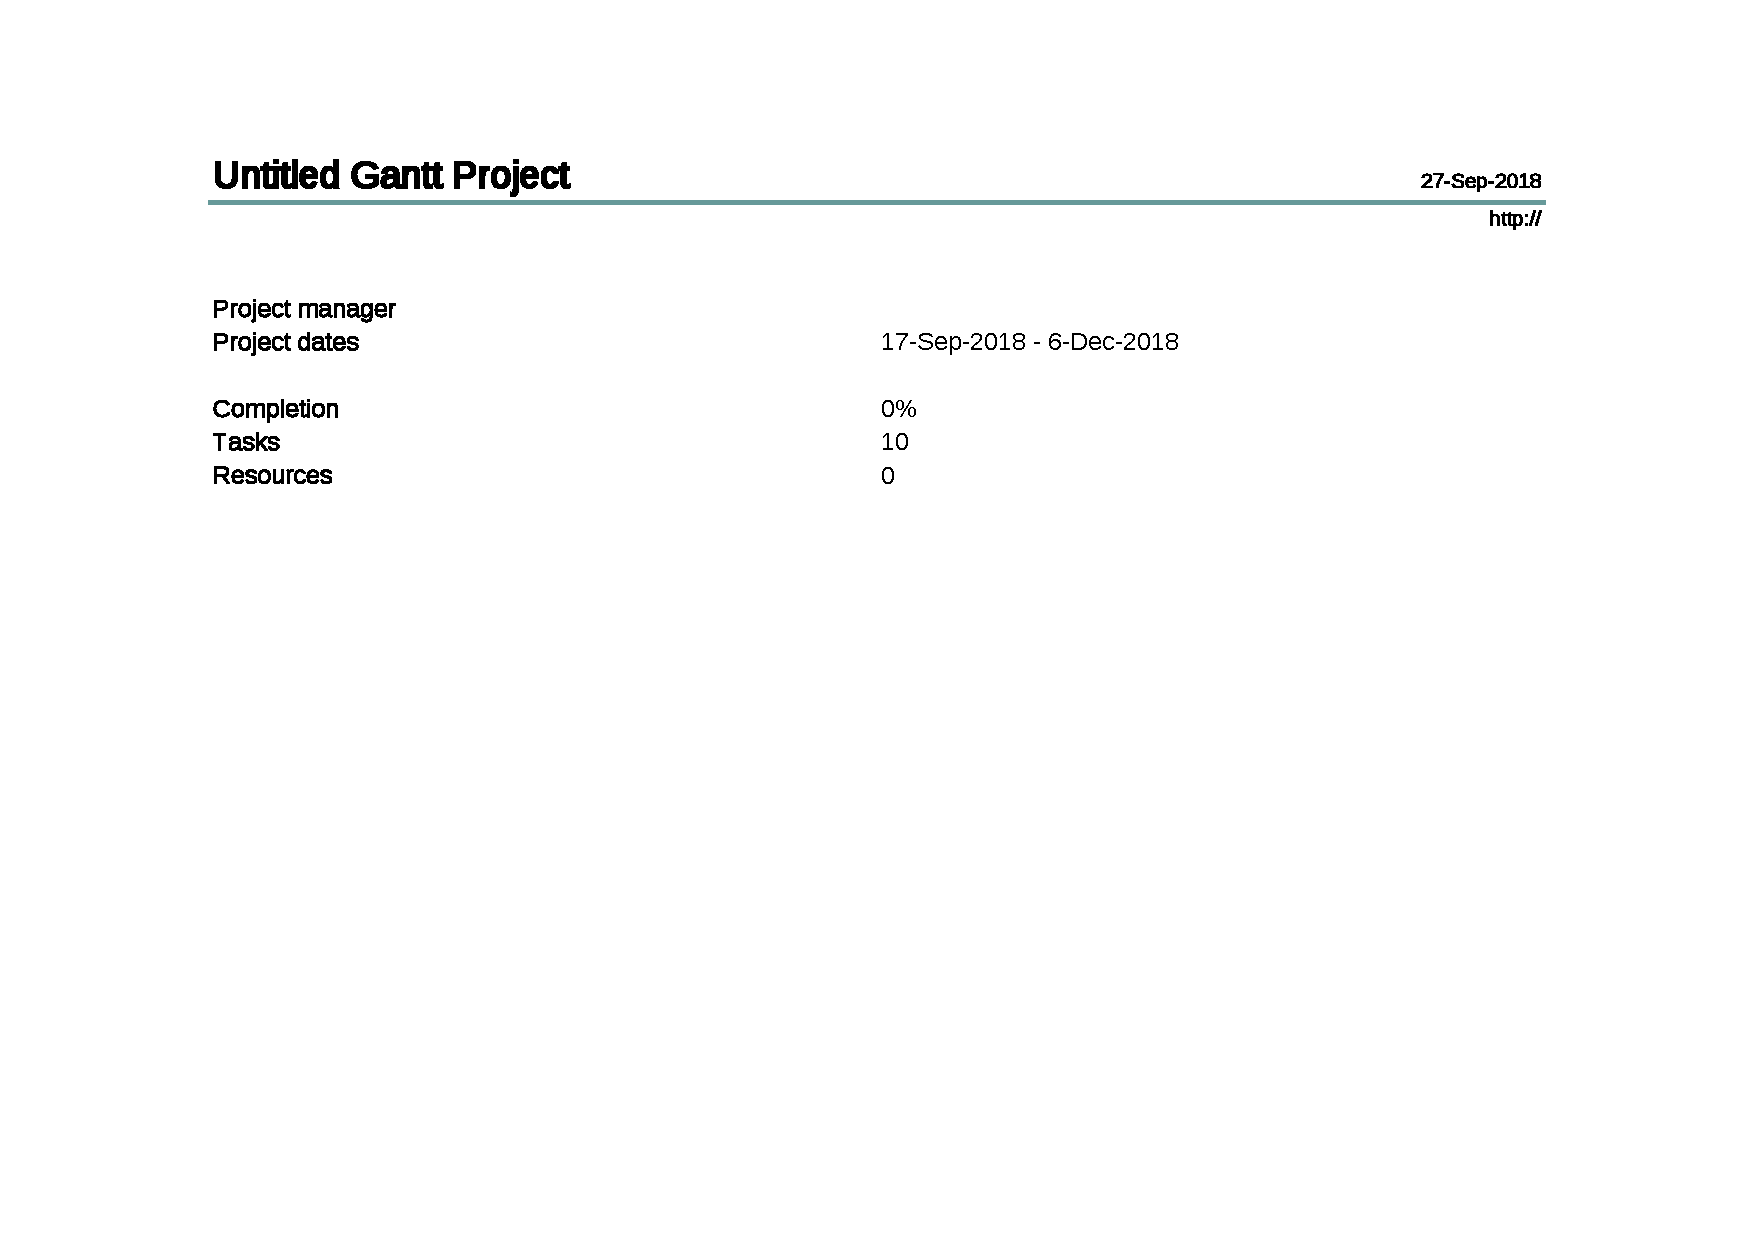
\includepdf[page={3}]{Gantt.pdf}

\section{Project Review}

\end{document}